
\subsection{Función de Rosembrock}

\subsubsection{2 dimensiones}

En la figura \ref{fig:rosembrock_2} se muestran los resultados de cada iteración obtenidos por la función de Rosembrock para el caso de $n=2$.

\begin{figure}[H]
    \centering
    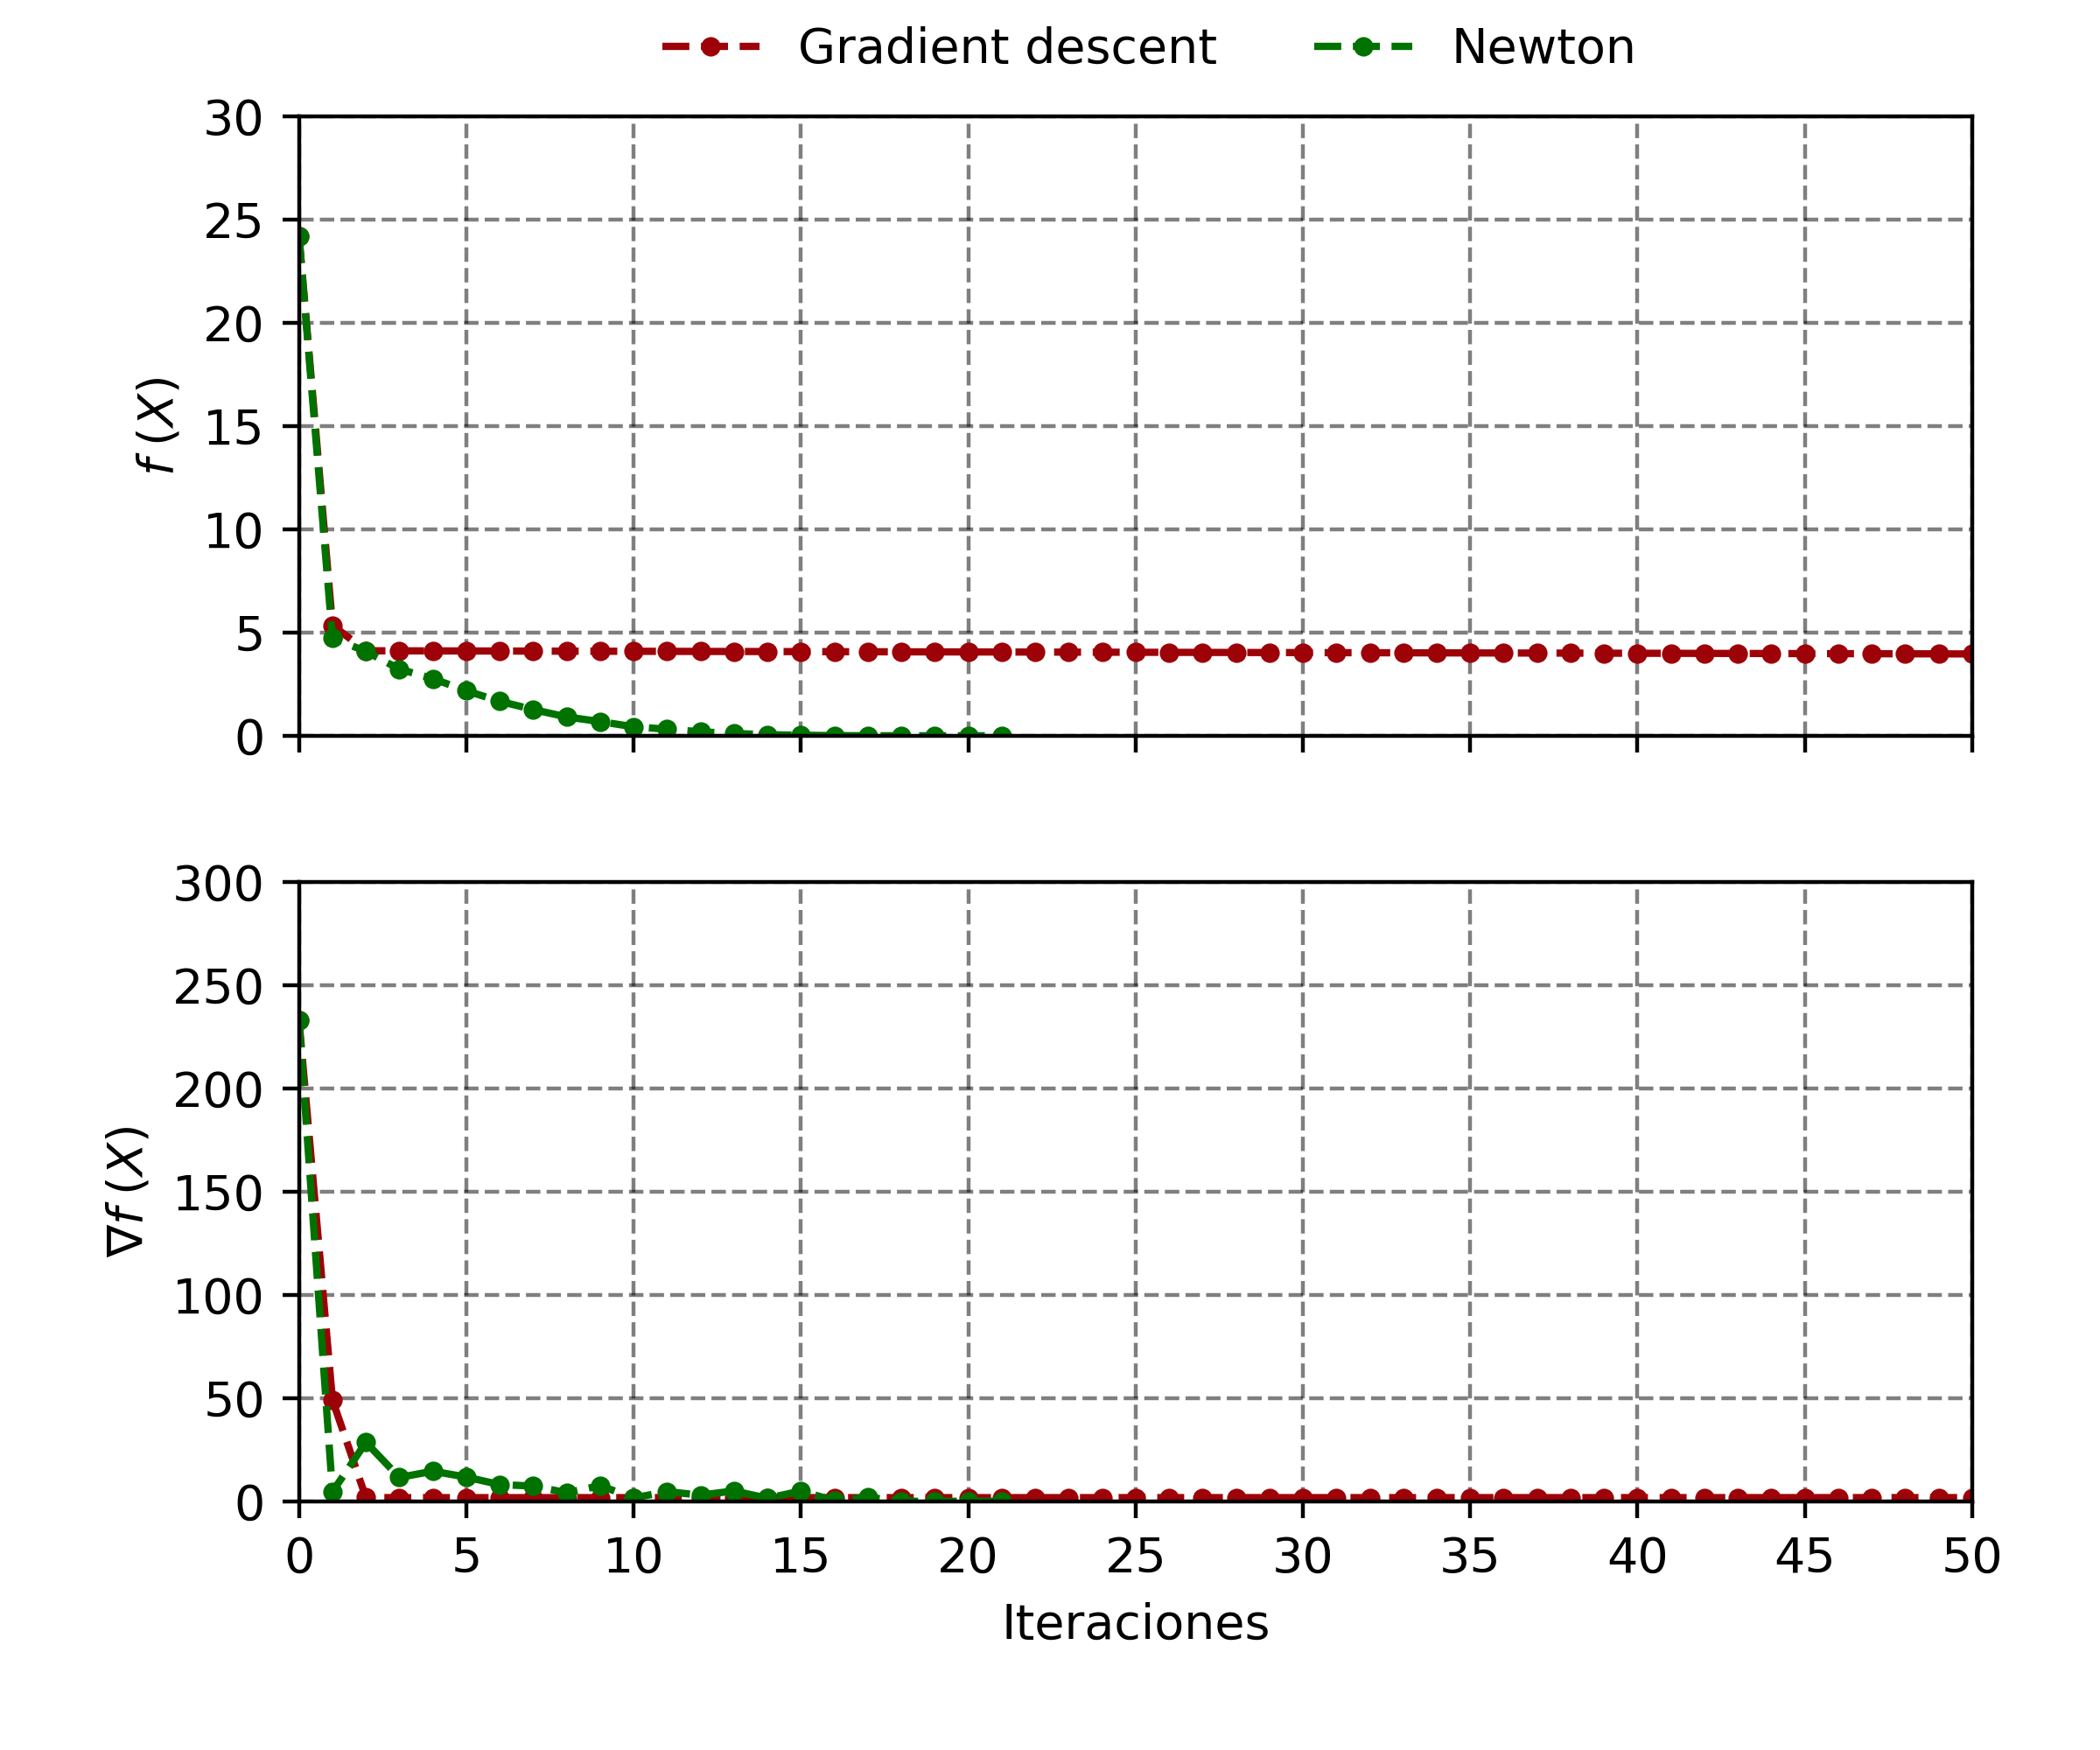
\includegraphics[width=12cm]{Graphics/Problema_2/rosembrock_2_predefined.png}
    \caption{Iteraciones de los métodos del descenso del gradiente y de Newton aplicados a la función de Rosembrock para n=2.}
    \label{fig:rosembrock_2}
\end{figure}

En la tabla \ref{table:rosembrock_2} se muestran los resultados de la primer y última iteracion para cada método.

\begin{table}[H]
    \centering
    \begin{tabular}{cccccc} \hline
        Método                 & Iteraciones & $f(x_0)$ & $f(x_n)$        & $\nabla f(x_0)$ & $\nabla f(x_n) $    \\ \hline
        Descenso del gradiente & 13931       & 24.2     & $0.000002$      & $232.8676$      & $0.001410$          \\
        Newton                 & 21          & 24.2     & $7.68x10^{-24}$ & $232.8676$      & $1.216668x10^{-10}$ \\ \hline
    \end{tabular}
    \caption{Resultados de la primer y última iteración del método del descenso del gradiente y de Newton para la función de Rosembrock para dos dimensiones.}
    \label{table:rosembrock_2}
\end{table}

\subsubsection{2 dimensiones con vector aleatorio}

En la figura \ref{fig:rosembrock_2_random} se muestran los resultados de cada iteración obtenidos por la función de Rosembrock para el caso de $n=2$.

\begin{figure}[H]
    \centering
    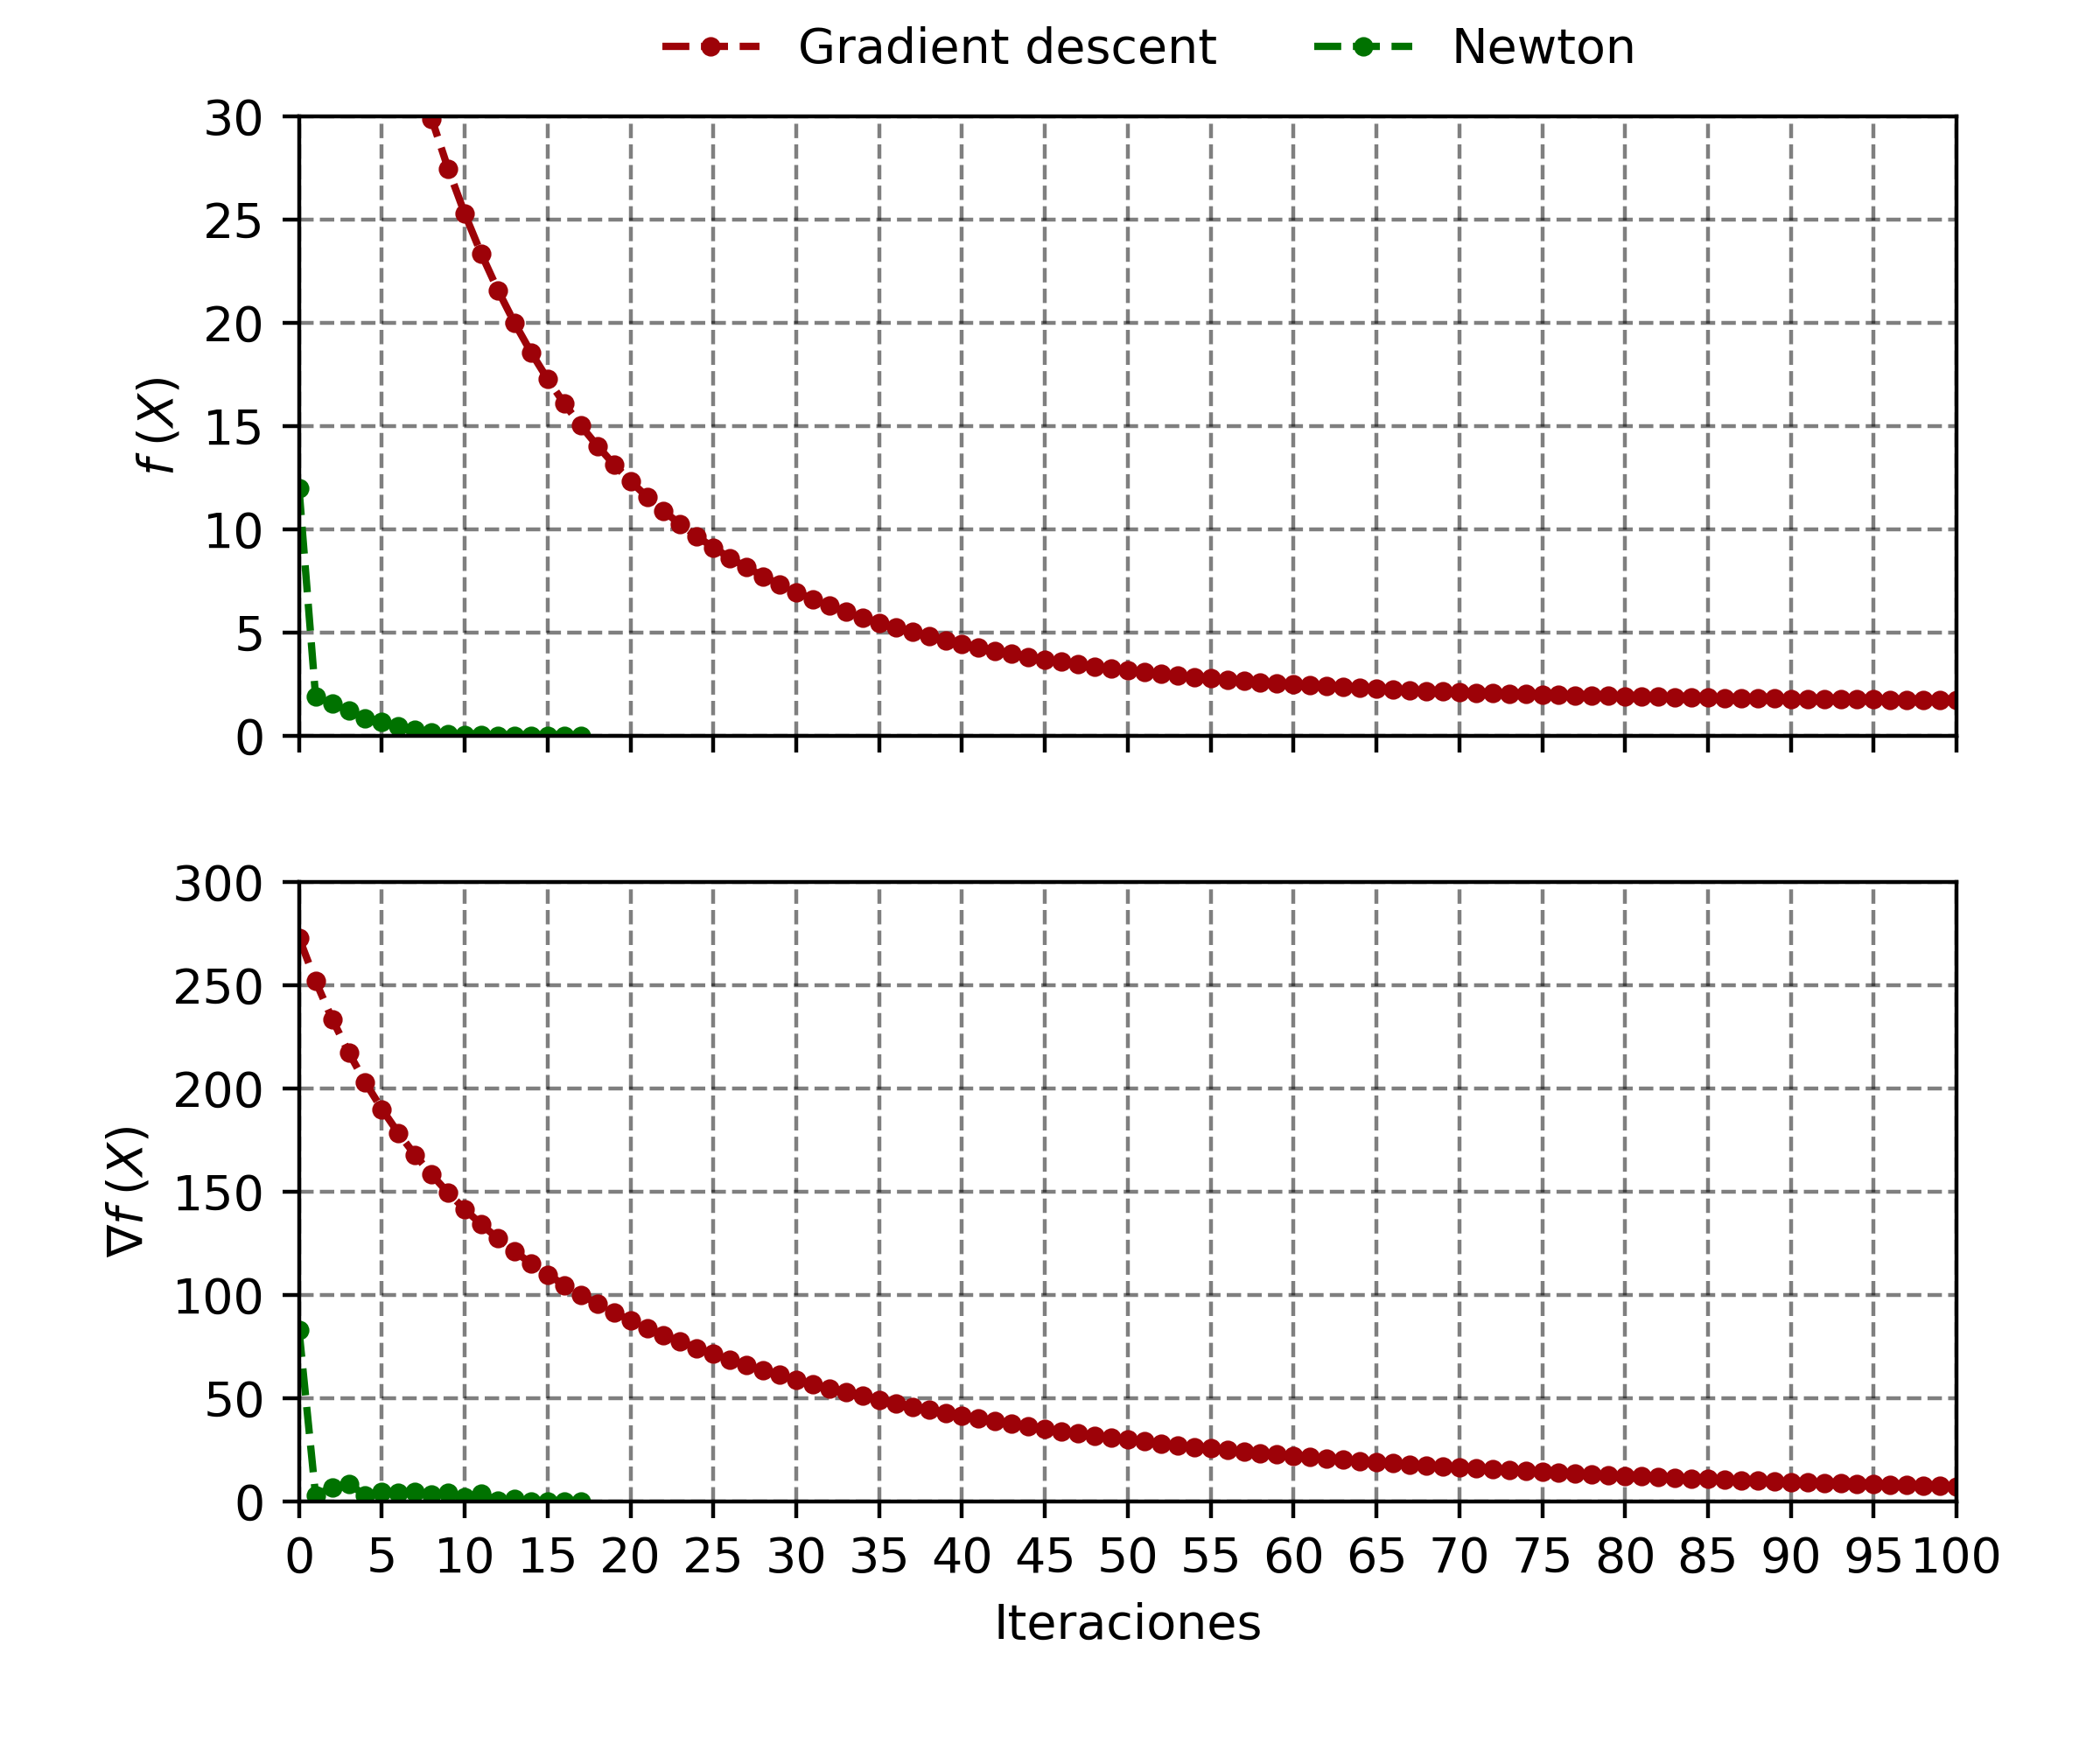
\includegraphics[width=12cm]{Graphics/Problema_2/rosembrock_2_random.png}
    \caption{Iteraciones de los métodos del descenso del gradiente y de Newton aplicados a la función de Rosembrock para n=2.}
    \label{fig:rosembrock_2_random}
\end{figure}

En la tabla \ref{table:rosembrock_2_random} se muestran los resultados de la primer y última iteracion para cada método.

\begin{table}[H]
    \centering
    \begin{tabular}{cccccc} \hline
        Método                 & Iteraciones & $f(x_0)$  & $f(x_n)$         & $\nabla f(x_0)$ & $\nabla f(x_n) $ \\ \hline
        Descenso del gradiente & 76754       & 66.316393 & $0.000233$       & $272.967314$    & $0.013819$       \\
        Newton                 & 17          & 11.98872  & $5.628x10^{-23}$ & $82.95111$      & $3.115x10^{-10}$ \\ \hline
    \end{tabular}
    \caption{Resultados de la primer y última iteración del método del descenso del gradiente y de Newton para la función de Rosembrock para dos dimensiones.}
    \label{table:rosembrock_2_random}
\end{table}

\subsubsection{100 dimensiones}

En la figura \ref{fig:rosembrock_100} se muestran los resultados de cada iteración obtenidos por la función de Rosembrock para el caso de $n=100$.

\begin{figure}[H]
    \centering
    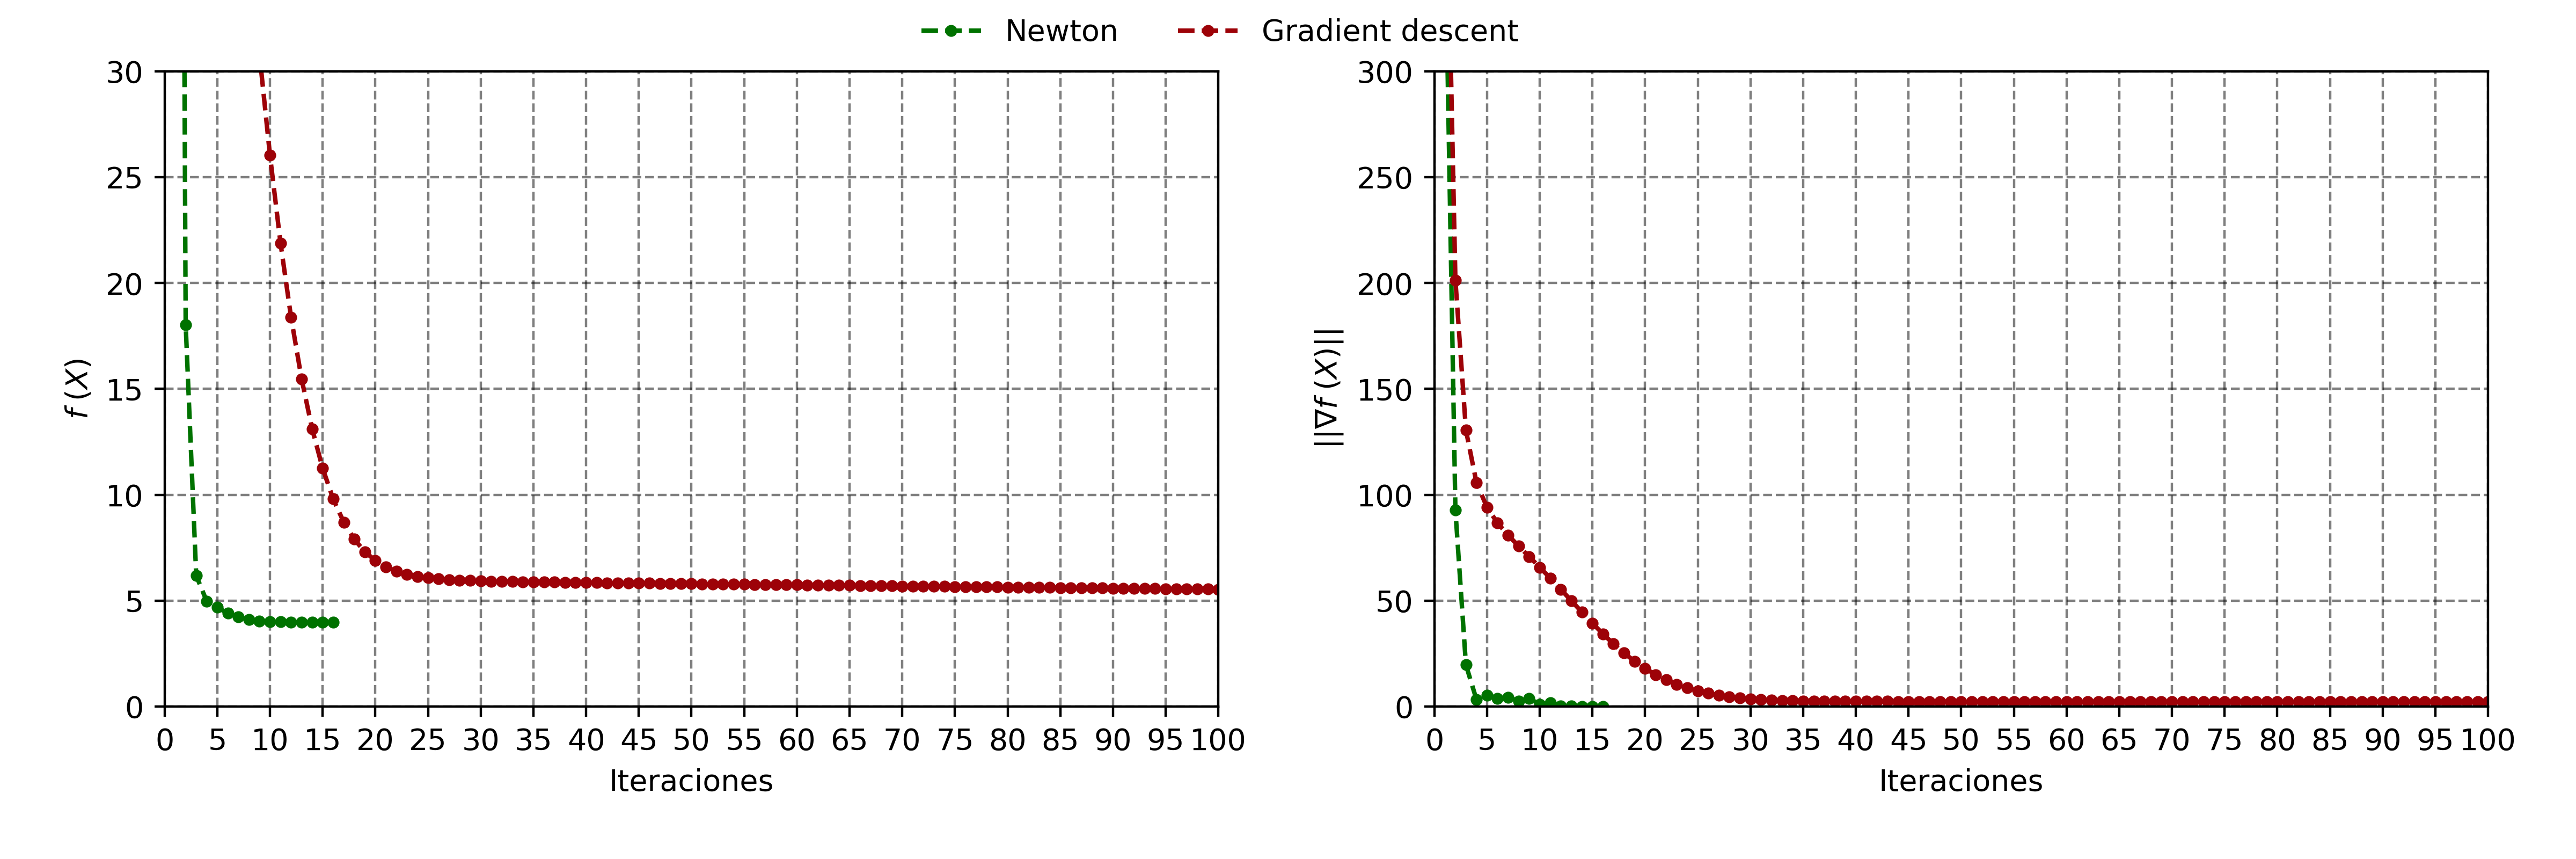
\includegraphics[width=12cm]{Graphics/Problema_2/rosembrock_100_predefined.png}
    \caption{Iteraciones de los métodos del descenso del gradiente y de Newton aplicados a la función de Rosembrock para n=100.}
    \label{fig:rosembrock_100}
\end{figure}

En la tabla \ref{table:rosembrock_100} se muestran los resultados de la primer y última iteracion para cada método.

\begin{table}[H]
    \centering
    \begin{tabular}{cccccc} \hline
        Método                 & Iteraciones & $f(x_0)$  & $f(x_n)$   & $\nabla f(x_0)$ & $\nabla f(x_n) $   \\ \hline
        Descenso del gradiente & $7337$      & $532.40 $ & $3.986624$ & $1125.2478$     & $0.009986$         \\
        Newton                 & $16$        & $532.40$  & $3.986624$ & $1125.2478$     & $3.15602x10^{-13}$ \\ \hline
    \end{tabular}
    \caption{Resultados de la primer y última iteración del método del descenso del gradiente y de Newton para la función de Rosembrock para 100 dimensiones.}
    \label{table:rosembrock_100}
\end{table}

\subsubsection{100 dimensiones con vector aleatorio}

En la figura \ref{fig:rosembrock_100_random} se muestran los resultados de cada iteración obtenidos por la función de Rosembrock para el caso de $n=100$.

\begin{figure}[H]
    \centering
    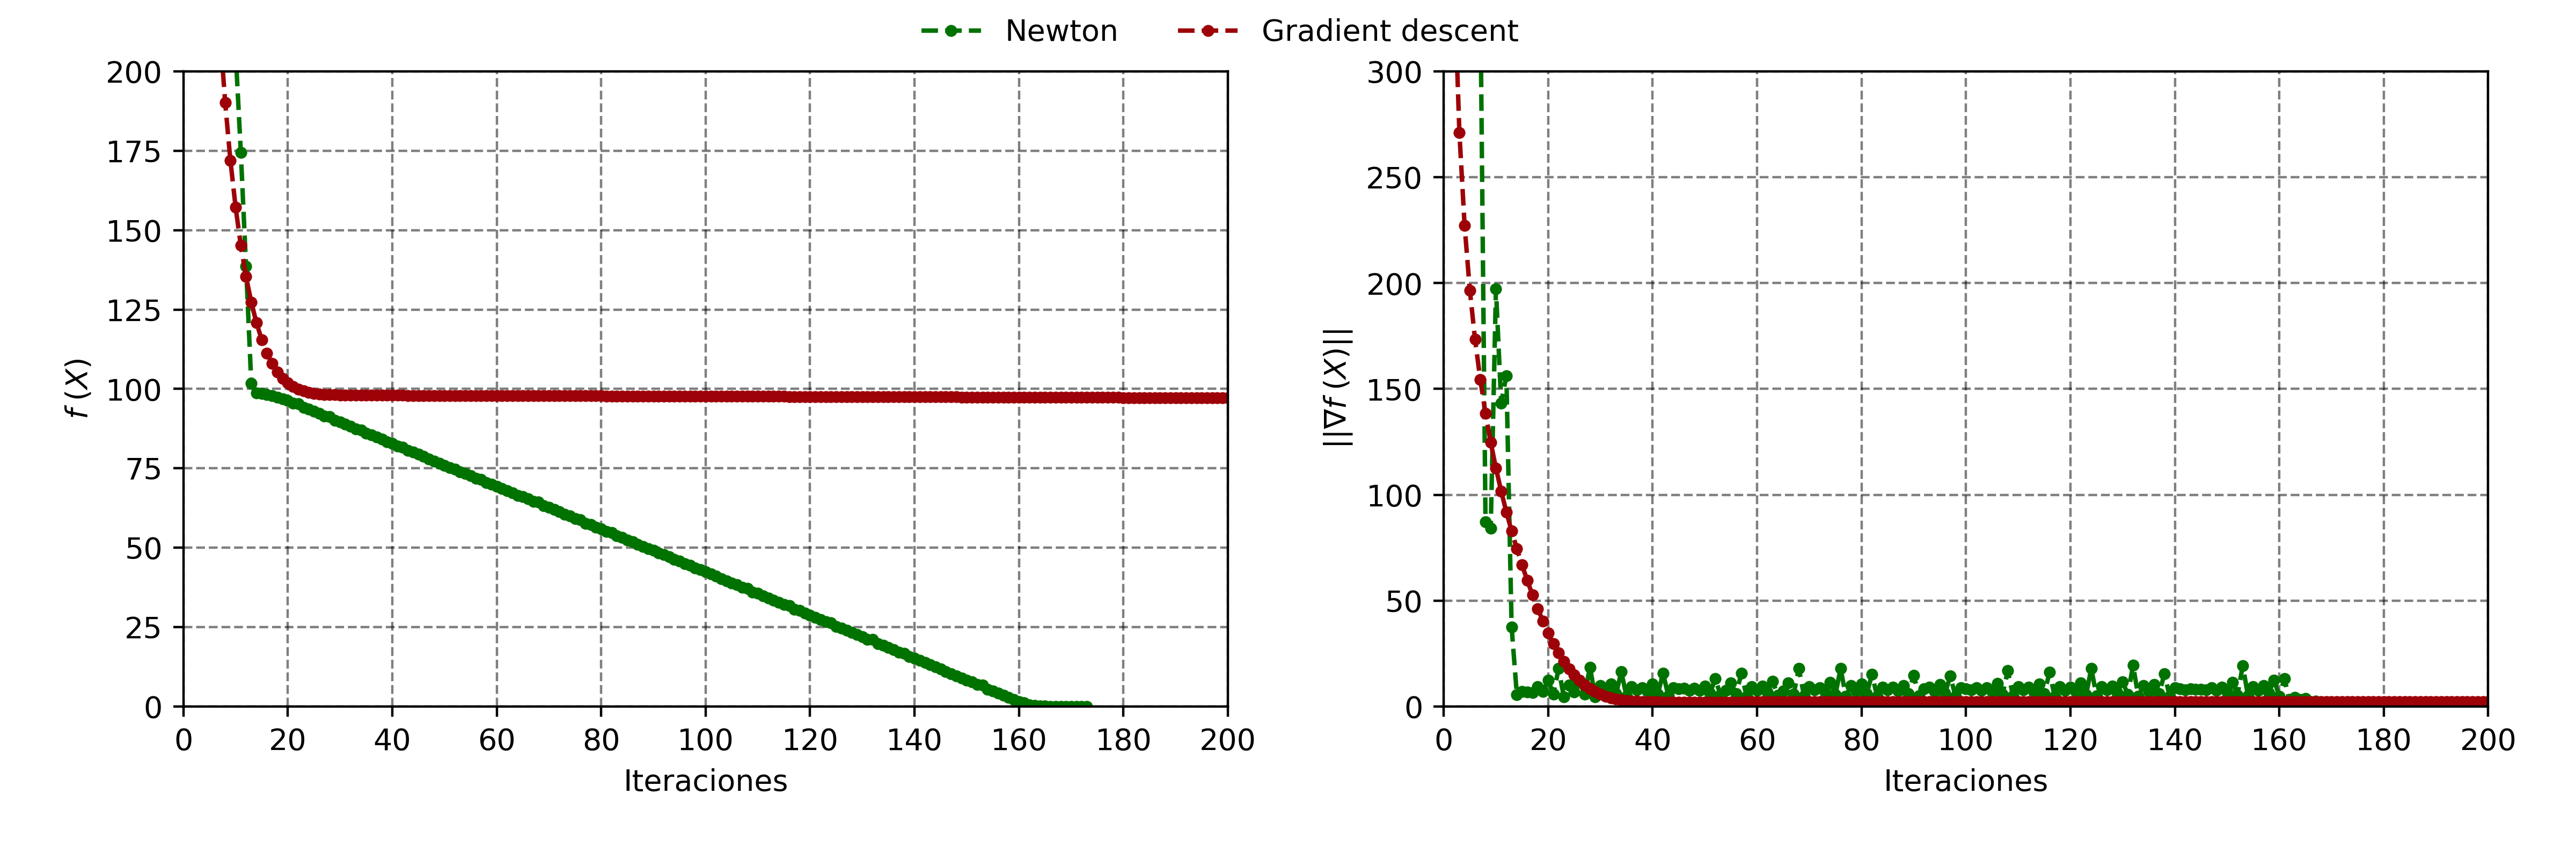
\includegraphics[width=12cm]{Graphics/Problema_2/rosembrock_100_random.png}
    \caption{Iteraciones de los métodos del descenso del gradiente y de Newton aplicados a la función de Rosembrock para n=100.}
    \label{fig:rosembrock_100_random}
\end{figure}

En la tabla \ref{table:rosembrock_100_random} se muestran los resultados de la primer y última iteracion para cada método.

\begin{table}[H]
    \centering
    \begin{tabular}{cccccc} \hline
        Método                 & Iteraciones & $f(x_0)$   & $f(x_n)$          & $\nabla f(x_0)$ & $\nabla f(x_n) $  \\ \hline
        Descenso del gradiente & $7337$      & $532.40 $  & $3.986624$        & $1125.2478$     & $0.009986$        \\
        Newton                 & $173$       & $3824.008$ & $7.5681x10^{-30}$ & $2682.654$      & $1.3651x10^{-13}$ \\ \hline
    \end{tabular}
    \caption{Resultados de la primer y última iteración del método del descenso del gradiente y de Newton para la función de Rosembrock para 100 dimensiones.}
    \label{table:rosembrock_100_random}
\end{table}

\subsubsection{Estadisticas con vectores aleatorios}

\paragraph{2 dimensiones}

\subparagraph{Método de Newton}

\begin{table}[H]
    \centering
    \begin{tabular}{ccc} \hline
                 & $f(x)$     & $||\nabla f(x)||$ \\ \hline
        n        & 100.000000 & 100.000000        \\
        Media    & 0.051269   & 0.189574          \\
        $\sigma$ & 0.300291   & 1.165927          \\
        Mínimo   & 0.000000   & 0.000000          \\
        Máximo   & 2.238695   & 8.806987          \\ \hline
    \end{tabular}
    \caption{Media, desviación estandar, mínimo y máximo de los resultados aleatorios usando el método de Newton en la función de Wood.}
    \label{table:rosembrock_4_random_newton}
\end{table}

\subparagraph{Método del descenso del gradiente}

\begin{table}[H]
    \centering
    \begin{tabular}{ccc} \hline
        {}       & $f(x)$              & $||\nabla f(x)||$   \\ \hline
        n        & 100                 & 100                 \\
        Media    & $2.333063x10^{-04}$ & $1.381915x10^{-02}$ \\
        $\sigma$ & $5.679958x10^{-09}$ & $1.702874x10^{-07}$ \\
        Mínimo   & $2.332966x10^{-04}$ & $1.381886x10^{-02}$ \\
        Máximo   & $2.333152x10^{-04}$ & $1.381942x10^{-02}$ \\ \hline
    \end{tabular}
    \caption{Media, desviación estandar, mínimo y máximo de los resultados aleatorios usando el método de Newton en la función de Wood.}
    \label{table:rosembrock_4_random_gradient}
\end{table}

\paragraph{100 dimensiones}

\subparagraph{Método de Newton}


\begin{table}[H]
    \centering
    \begin{tabular}{ccc} \hline
                 & $f(x)$      & $||\nabla f(x)||$ \\ \hline
        n        & 100.000000  & 100.000000        \\
        Media    & 426.440128  & 290.794079        \\
        $\sigma$ & 1002.282274 & 722.327174        \\
        Mínimo   & 0.000000    & 0.000000          \\
        Máximo   & 5344.705735 & 3423.160112       \\ \hline
    \end{tabular}
    \caption{Media, desviación estandar, mínimo y máximo de los resultados aleatorios usando el método de Newton en la función de Wood.}
    \label{table:rosembrock_100_random_newton}
\end{table}

\subparagraph{Método del descenso del gradiente}

\begin{table}[H]
    \centering
    \begin{tabular}{ccc} \hline
                 & $f(x)$             & $||\nabla f(x)||$  \\ \hline
        n        & 100                & 100                \\
        Media    & $2.391974x10^{-1}$ & $9.992327x10^{-5}$ \\
        $\sigma$ & $9.515404x10^{-1}$ & $1.602367x10^{-8}$ \\
        Mínimo   & $1.000360x10^{-8}$ & $9.988768x10^{-5}$ \\
        Máximo   & $3.986624$         & $9.994944x10^{-5}$ \\ \hline
    \end{tabular}
    \caption{Media, desviación estandar, mínimo y máximo de los resultados aleatorios usando el método de Newton en la función de Wood.}
    \label{table:rosembrock_100_random_gradient}
\end{table}